% !TEX options=--shell-escape
\documentclass [12pt]{article} 
\usepackage {amsmath}
\usepackage {amsthm}
\usepackage {amssymb}
\usepackage {graphicx} 
\usepackage {float}
\usepackage {multirow}
\usepackage {xcolor}
\usepackage {algorithmic}
\usepackage [ruled,vlined,commentsnumbered,titlenotnumbered]{algorithm2e} \usepackage {array} 
\usepackage {booktabs} 
\usepackage {url} 
\usepackage {parskip} 
\usepackage [margin=1in]{geometry} 
\usepackage [T1]{fontenc} 
\usepackage {cmbright} 
\usepackage [many]{tcolorbox} 
\usepackage [colorlinks = true,
            linkcolor = blue,
            urlcolor  = blue,
            citecolor = blue,
            anchorcolor = blue]{hyperref} 
\usepackage {enumitem} 
\usepackage {xparse} 
\usepackage {verbatim}
\usepackage{listings}
\usepackage{xcolor}
\usepackage{csquotes}
\usepackage[cache=false]{minted}
\usepackage{mdframed}
\usepackage{tikz}
\usetikzlibrary{shapes.symbols}
\newtheorem{theorem}{Theorem}

\DeclareTColorBox {Solution}{}{breakable, title={Solution}}
\DeclareTColorBox {Solution*}{}{breakable, title={Solution (provided)}}
\DeclareTColorBox {Instruction}{}{boxrule=0pt, boxsep=0pt, left=0.5em, right=0.5em, top=0.5em, bottom=0.5em, arc=0pt, toprule=1pt, bottomrule=1pt}
\DeclareDocumentCommand {\Expecting }{+m}{\textbf {[We are expecting:} #1\textbf {]}}
\DeclareDocumentCommand {\Points }{m}{\textbf {(#1 pt.)}} 
\newcommand {\hint }[1]{\noindent {[\textbf {HINT:} \em #1 \em ]}} \newcommand {\pts }[1]{\textbf {(#1 pt.)}} 

\begin{document} 

{\LARGE \textbf {COMP 285 (NC A\&T, Spr `22)}\hfill \textbf {Weekly Quiz 5} } 

\begin{Instruction}

\paragraph{Reporting Issues} If you find any issues with the solutions, reach out to Chi Wang (author) or Luis Perez (reviewer).

\end{Instruction}


\section{} In order to conclude an expected runtime of $O(1)$ for hash table operations, we assumed the followingtwo happen in some specific order: 
\begin{enumerate}
    \item The adversary picks elements $x_1, \cdots , x_n$ for the hash table
    \item The algorithm picks a hash function from the hash family.
\end{enumerate}

\begin{Solution}
(1) Adversary first, then (2) algorithm.
\paragraph{}

Bad guys may lower our running time by picking the worst-case element if they know the hash function algorithm before picking elements. 
\end{Solution}


\section{} Math review: What is $285 \mod 5$?

\begin{Solution}
0
\end{Solution}


\section{} Math review: What is the meaning of the ``$a \mod b$'' operation?

\begin{Solution}
You divide $a$ by $b$ and take the remainder.
\end{Solution}


\section{} Suppose that we have a universe of size $M$, and our hash table size is $n$. If $n \geq M$, what is the minimum size of a universal hash family?

\begin{Solution}
1
\paragraph{}
Since our hash table is bigger than our universe, a single hash function will be sufficient for the family to be universal.
\end{Solution}


\section{} You start your DFS algoritmh at node $0$, and assume that the vertices' numbers are used as tie breakers (you visit vertices with smaller numbers first). In what order do you enter the vertices.
\begin{figure}[H]
    \centering
    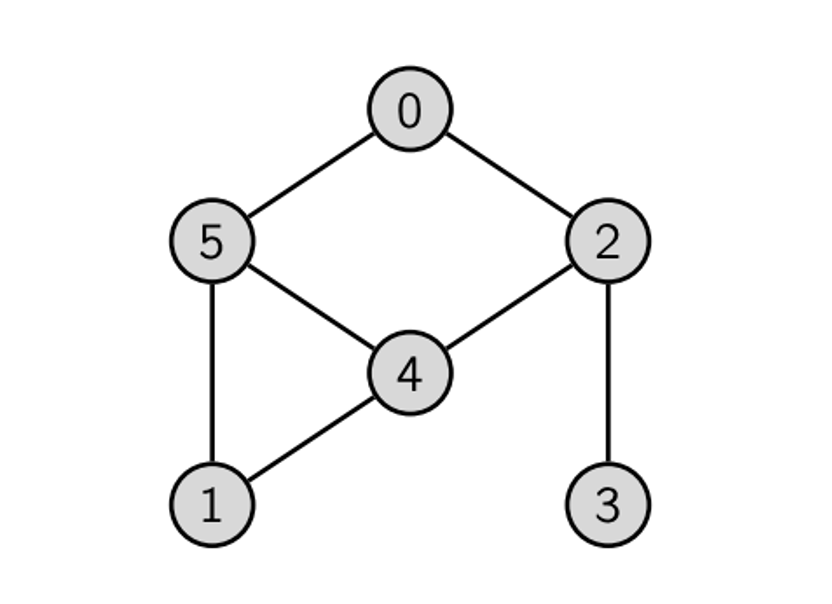
\includegraphics[scale=0.5]{1.png} 
    \label{fig:my_label}
\end{figure}

\begin{Solution}
0, 2, 3, 4, 1, 5
\end{Solution}


\section{} You start your DFS algoritmh at node 0, and assume that the vertices' numbers are used as tie breakers (you visit vertices with larger numbers first). In what order do you enter the vertices. 
\begin{figure}[H]
    \centering
    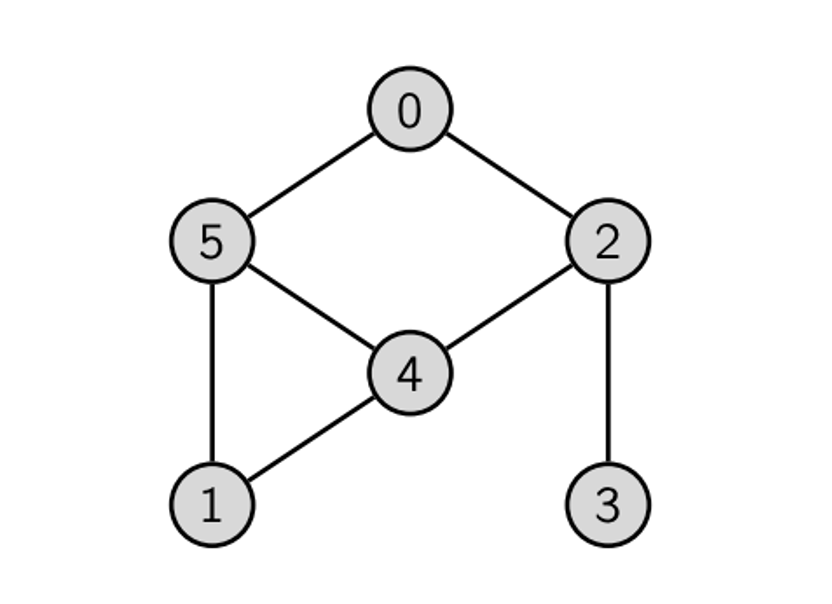
\includegraphics[scale=0.5]{1.png} 
    \label{fig:my_label}
\end{figure}

\begin{Solution}
0, 5, 4, 2, 3, 1
\end{Solution}


\section{} What is the degree of vertex 4?
\begin{figure}[H]
    \centering
    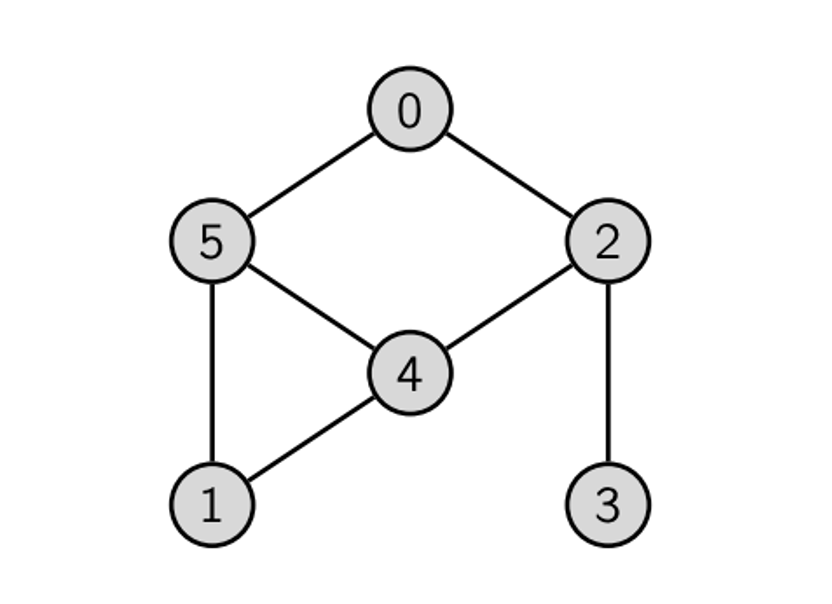
\includegraphics[scale=0.5]{1.png} 
    \label{fig:my_label}
\end{figure}

\begin{Solution}
3
\paragraph{}
There are 3 edges coming out from the vertex 4.
\end{Solution}


\section{} Two options for representing graphs are the (1) adjacency list representations and the (2) matrix representation. For edge (v, w), what is the running time of checking if it exists in the matrix representation, where $n$ is the number of nodes in the graph? There may be multiple correct answers. Select 1.

\begin{Solution}
$O(1)$
\paragraph{}
Simply check $matrix[v][w]$, 1 or 0 means there exists such edge or not. 
\end{Solution}


\section{} Two options for representing graphs are the (1) adjacency list representations and the (2) matrix representation. For edge (v, w), what is the running time of checking if it exists in the adjacency list representation, where n is the number of nodes in the graph? There may be multiple correct answers. Select 1.

\begin{Solution}
$O(\text{degree}(v)) / O(\text{degree}(w))$
\paragraph{}
To find edge(v,w), we may need to iterate the whole list whose size is $\text{degree}(v)/\text{degree}(w)$.
\end{Solution}


\section{} Two options for representing graphs are the (1) adjacency list representations and the (2) matrix representation. How much space is required for each, where n is the number of nodes and m is the number of edges. 

\begin{Solution}
Adjacency: $O(n+m)$, Matrix: $O(n^2)$
\end{Solution}


















\end{document} 